\documentclass[a4paper,11pt]{article}
\usepackage{ctex}
\usepackage{enumerate}
\usepackage{times}
\usepackage{mathptmx}
\usepackage{amsmath}
\usepackage{amssymb}
\usepackage{tikz}
\usepackage{clrscode3e}
\usepackage[top=2cm, bottom=2cm, left=2cm, right=2cm]{geometry}

\allowdisplaybreaks[4]
\renewcommand{\labelenumi}{\textbf{\emph{\alph{enumi}}.}}
\newcommand{\NIL}{\const{nil}}
\begin{document}
  \title{����~2-14~��ҵ}
  \author{��������ۿԴ \and ѧ�ţ�161240004}
  \date{}
  \maketitle

  \section{[TC] Problem 21.1-2}
  ``If'': we use mathematical induction to prove this. For base step, $a$ and $a$ are in the same set, and $a$ and $a$ are in the same connected component. For induction step, if $S$ is a set, then $S$ is either a set with only one element, or a set which is a union of two disjoint sets, say $S_1$ and $S_2$, connected by edge $(u, v)$ where $u \in S_1$ and $v \in S_2$. In the latter case, for every two elements $x$ and $y$ in $S$, if both $x$ and $y$ are in $S_1$ or $S_2$, then $x$ and $y$ are in the same connected component by induction hypothesis. Otherwise, assume $x \in S_1$, $y \in S_2$, then $x$ has a path to $u$, $v$ has a path to $v$, and there exists edge $(u, v)$, thus $x$ and $y$ are connected. Therefore, if two elements are in the same set, they are in the same connected component. \par
  ``Only if'': if $a$ and $b$ are in the same connected component, then there exists a path from $a$ to $b$. After the procedure executed, all edges in the path have been processed and all these vertices have been united, thus $a$ and $b$ are in the same set.

  \section{[TC] Problem 21.1-3}
  There are $|E|$ edges in the graph, and for every edge, \proc{Find-Set} is called twice, thus \proc{Find-Set} is called $2|E|$ times in all. \par
  The edges, where \proc{Union} is performed, constitute the spanning trees of the connected components. For the $i$th connected component, assume there are $|V_i|$ vertices, then its spanning tree has $|V_i|-1$ edges. Therefore, there are $|V| - k$ edges in the spanning trees, so \proc{Union} is called $|V| - k$ times in all.

  \section{[TC] Problem 21.2-1}
  \begin{codebox}
  \Procname{$\proc{Make-Set}(x)$}
  \li let $S$ be new linked list
  \li $\attrib{S}{head} \gets x$
  \li $\attrib{S}{tail} \gets x$
  \li $\attrib{S}{weight} \gets 1$
  \li $\attrib{x}{root} \gets S$
  \li $\attrib{x}{next} \gets \NIL$
  \end{codebox}

  \begin{codebox}
  \Procname{$\proc{Find-Set}(x)$}
  \li \Return $\attribb{x}{root}{head}$
  \end{codebox}

  \begin{codebox}
  \Procname{$\proc{Union}(x, y)$}
  \li \If $\attrib{x}{weight} < \attrib{y}{weight}$ \Then
  \li     swap $x$ and $y$
      \End
  \li $t \gets \attrib{y}{head}$
  \li \While $t \neq \NIL$
  \li \Do $\attrib{t}{root} \gets x$
  \li     $t \gets \attrib{t}{next}$
      \End
  \li $\attribb{x}{tail}{next} \gets \attrib{y}{head}$
  \li $\attrib{x}{tail} \gets \attrib{y}{tail}$
  \li $\attrib{x}{weight} \gets \attrib{x}{weight} + \attrib{y}{weight}$
  \end{codebox}

  \section{[TC] Problem 21.2-3}
  It is obvious that \proc{Make-Set} and \proc{Find-Set} take an amortized running time of $O(1)$. We have proved in Theorem 21.1, that we perform at most $n-1$ \proc{Union} operations over all, and the total time spent on \proc{Union} is $O(n \lg n)$. Thus the amortized running time of \proc{Union} is $O(\lg n)$.

  \section{[TC] Problem 21.2-6}
  \begin{codebox}
  \Procname{$\proc{Union}(x, y)$}
  \zi \Comment if weighted-union heuristic is used
  \li \If $\attrib{x}{weight} < \attrib{y}{weight}$ \Then
  \li     swap $x$ and $y$
      \End
  \li $t \gets \attrib{y}{head}$
  \li \While $\attrib{t}{next} \neq \NIL$
  \li \Do $\attrib{t}{root} \gets x$
  \li     $t \gets \attrib{t}{next}$
      \End
  \li $\attrib{t}{root} \gets x$
  \li $\attrib{t}{next} \gets \attrib{x}{head}$
  \li $\attrib{x}{head} \gets \attrib{y}{head}$
  \end{codebox}

  \section{[TC] Problem 21.3-1}
  \scriptsize
  \begin{centering}
  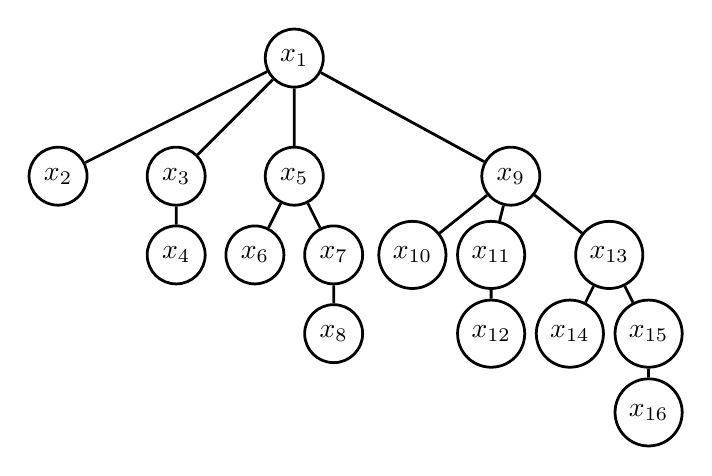
\begin{tikzpicture}[line width = 1pt,
                    solid/.style = {circle, draw, fill = black, minimum size = 0.3cm},
                    empty/.style = {circle, draw, fill = white, minimum size = 0.3cm}]
  \node [empty] (T1) at (0, 0) {$x_1$};
  \node [empty] (T2) at (-3, -1.5) {$x_2$};
  \node [empty] (T3) at (-1.5, -1.5) {$x_3$};
  \node [empty] (T4) at (-1.5, -2.5) {$x_4$};
  \node [empty] (T5) at (0, -1.5) {$x_5$};
  \node [empty] (T6) at (-0.5, -2.5) {$x_6$};
  \node [empty] (T7) at (0.5, -2.5) {$x_7$};
  \node [empty] (T8) at (0.5, -3.5) {$x_8$};
  \node [empty] (T9) at (2.75, -1.5) {$x_9$};
  \node [empty] (T10) at (1.5, -2.5) {$x_{10}$};
  \node [empty] (T11) at (2.5, -2.5) {$x_{11}$};
  \node [empty] (T12) at (2.5, -3.5) {$x_{12}$};
  \node [empty] (T13) at (4, -2.5) {$x_{13}$};
  \node [empty] (T14) at (3.5, -3.5) {$x_{14}$};
  \node [empty] (T15) at (4.5, -3.5) {$x_{15}$};
  \node [empty] (T16) at (4.5, -4.5) {$x_{16}$};
  \draw (T1) -- (T2);
  \draw (T1) -- (T3) -- (T4);
  \draw (T1) -- (T5) -- (T6);
  \draw (T5) -- (T7) -- (T8);
  \draw (T1) -- (T9) -- (T10);
  \draw (T9) -- (T11) -- (T12);
  \draw (T9) -- (T13) -- (T14);
  \draw (T13) -- (T15) -- (T16);
  \end{tikzpicture} \par
  \end{centering}
  \normalsize
  The answers returned by the \proc{Find-Set} operations is $x_1$.

  \section{[TC] Problem 21.3-2}
  \begin{codebox}
  \Procname{$\proc{Find-Set}(x)$}
  \li $y \gets x$
  \li \While $\attrib{y}{p} \neq y$
  \li \Do $y \gets \attrib{y}{p}$
      \End
  \li $z \gets x$
  \li \While $z \neq y$
  \li \Do $x \gets \attrib{z}{p}$
  \li     $\attrib{z}{p} \gets y$
  \li     $z \gets x$
      \End
  \li \Return $y$
  \end{codebox}

  \section{[TC] Problem 21.3-3}
  Assume $A[0 \cdots n-1]$ is an array of elements. The sequence is given by the following procedure. \par
  \begin{codebox}
  \li \For $i \gets 0$ \To $n-1$
  \li \Do $\proc{Make-Set}(x_i)$
      \End
  \li $j \gets 2$
  \li \While $j < n$
  \li \Do \For $i \gets 0$ \To $n$ \By $j$
  \li     \Do  \If $i+j/2 < n$ \Then
  \li              $\proc{Union}(x_i, x_{i+j/2})$
               \End
          \End
  \li    $j \gets 2j$
      \End
  \li $t \gets 2^{\lfloor \lg n \rfloor} - 1$
  \li \For $i \gets 1$ \To $m - 2n + 1$
  \li \Do  $\proc{Find-Set}(x_t)$
      \End
  \end{codebox} \par
  Each iteration of \While (except the last one if $n$ is not a power of 2) in line 4-8 increments the depth of $x_t$ by 1. So the depth of $x_t$ is $\lfloor \lg n \rfloor$ at last. There are $n$ calls to \proc{Make-Set} and $n-1$ calls to \proc{Union}, each taking $\Omega(1)$ time. The $m - 2n + 1$ calls to \proc{Find-Set} take $\Omega(\lg n)$ time each. The total running time is $\Omega(2n-1 + (m-2n+1) \lg n)$, and if $m = \omega(n)$, it is $\Omega(m \lg n)$.

  \section{[TC] Problem 21-1}
  \begin{enumerate}
  \item $\{4, 3, 2, 6, 8, 1\}$
  \item We use the following loop invariant to prove the correctness:
  \begin{quote}
    Before each iteration of \For loop, for every $j$, $extracted[j]$ is either empty, or filled with correct value; if it is empty, then��
    \begin{enumerate}[(1)]
    \item the correct value of $extracted[j]$ is greater than or equal to $i$, or the set is empty when the corresponding \proc{Extract-Min} is called;
    \item $K_j$ exists and $K_j = \cap_{i=k}^{j} I_j$, where $k$ is the minimum of $l$ such that for every $i$ between $l$ and $j$, either $i = j$ or $extracted[i]$ has been filled with correct value. (this is also true for $j = m+1$)
    \end{enumerate}
  \end{quote}
  \textbf{Initialization:} Prior to the first iteration, all elements of $extracted$ is empty, and both (1) and (2) are correct for every $j$. \par
  \textbf{Maintenance:} During the iteration, if $j = m + 1$, by loop invariant (2), there is no unprocessed \proc{Extract-Min} after $i$ in the original sequence, and the loop invariant holds. If $j \neq m + 1$, there exist some unprocessed \proc{Extract-Min}s after $i$ in the original sequence, among which the first one to appear is $j$, according to loop invariant (2). By loop invariant (1), $extracted[j]$ must be $i$. Line 7 maintains the loop invariant (2). Therefore, the loop invariant still holds after each iteration.\par
  \textbf{Termination:} When the loop terminates, $i \gets n+1$. For every $j$, if $extracted[j]$ is empty, the set must be empty when the corresponding \proc{Extract-Min} is called, because the correct value of $extracted[j]$ can't be greater than or equal to $n+1$. Thus, the array $extracted$ returned by \proc{Off-Line-Minimum} is correct.
  \item To find the smallest value greater than $j$ for which set $K_l$ exists quickly, we shall maintain a linked list of the sets. When $K_j$ is destroyed, the set should be deleted from the list. It takes $O(m)$ time to build the list, and $O(1)$ time to delete an element. There are $n$ itertaions, and every element of $extracted$ is filled at most once, which takes an amortized running time of $O(\alpha(n))$, if both union by rank and path compression are used. Thus, the total running time if $O(n + m \alpha(n))$.
  \end{enumerate}

\end{document}
